\label{key}\chapter{Podsumowanie}
\label{cha:elementyPracyproj}
\section{Podsumowanie ogólne}
Projekt zakładał stworzenie aplikacji desktopowej wspomagającej zarządzanie zamówieniami w kolejce FIFO. Osiągnięto wszystkie założone cele, w tym poprawne działanie kolejki, zapis i odczyt danych z bazy oraz prosty graficzny interfejs.

% ********************
Możliwości rozwoju:
\begin{itemize}
    \item logowanie użytkowników
    \item generowanie faktur PDF
    \item Rozdzielenie bazy danych, przechowującej klientów, produkty oraz Zamówienia.
    \item Pokazywanie ilości produktów w magazynie.
    \item Integrację z systemem wysyłek.
    \item W przypadku braku produktu, na półkach, uniemożliwienie jego zakupu.
\end{itemize}


\section{Harmonogram realizacji projektu}

\begin{figure}[H]
	\centering
	\includegraphics[width=0.7\linewidth]{../../Downloads/diagram_gantta}
	\caption{Harmonogram realizacji projektu}
	\label{fig:diagramgantta}
\end{figure}


\section{Wnioski}

Projekt udowadnia, że przy użyciu podstawowych narzędzi Javy można stworzyć w pełni działający
system do zarządzania zamówieniami, z czytelnym GUI oraz trwałym przechowywaniem danych. Kod jest
modularny, co ułatwia jego dalszy rozwój i integrację z innymi systemami. Istnieje jednak kilka opcji rozwoju programu w kierunku bardziej zaawansowanego narzęcia do zarządzania w bardziej profesjonalny sposób zakupami, stanem magazynu m.in: Przez dodanie stanów magazynów, możliwość logowania, zarówno pracowników jak i klientów.


\section{Oświadczenie studenta o samodzielności pracy}

Oświadczenie należy wydrukować, podpisać, zeskanować i umieścić jako załącznik do niniejszej dokumentacji.

\begin{figure}[H]
	\centering
	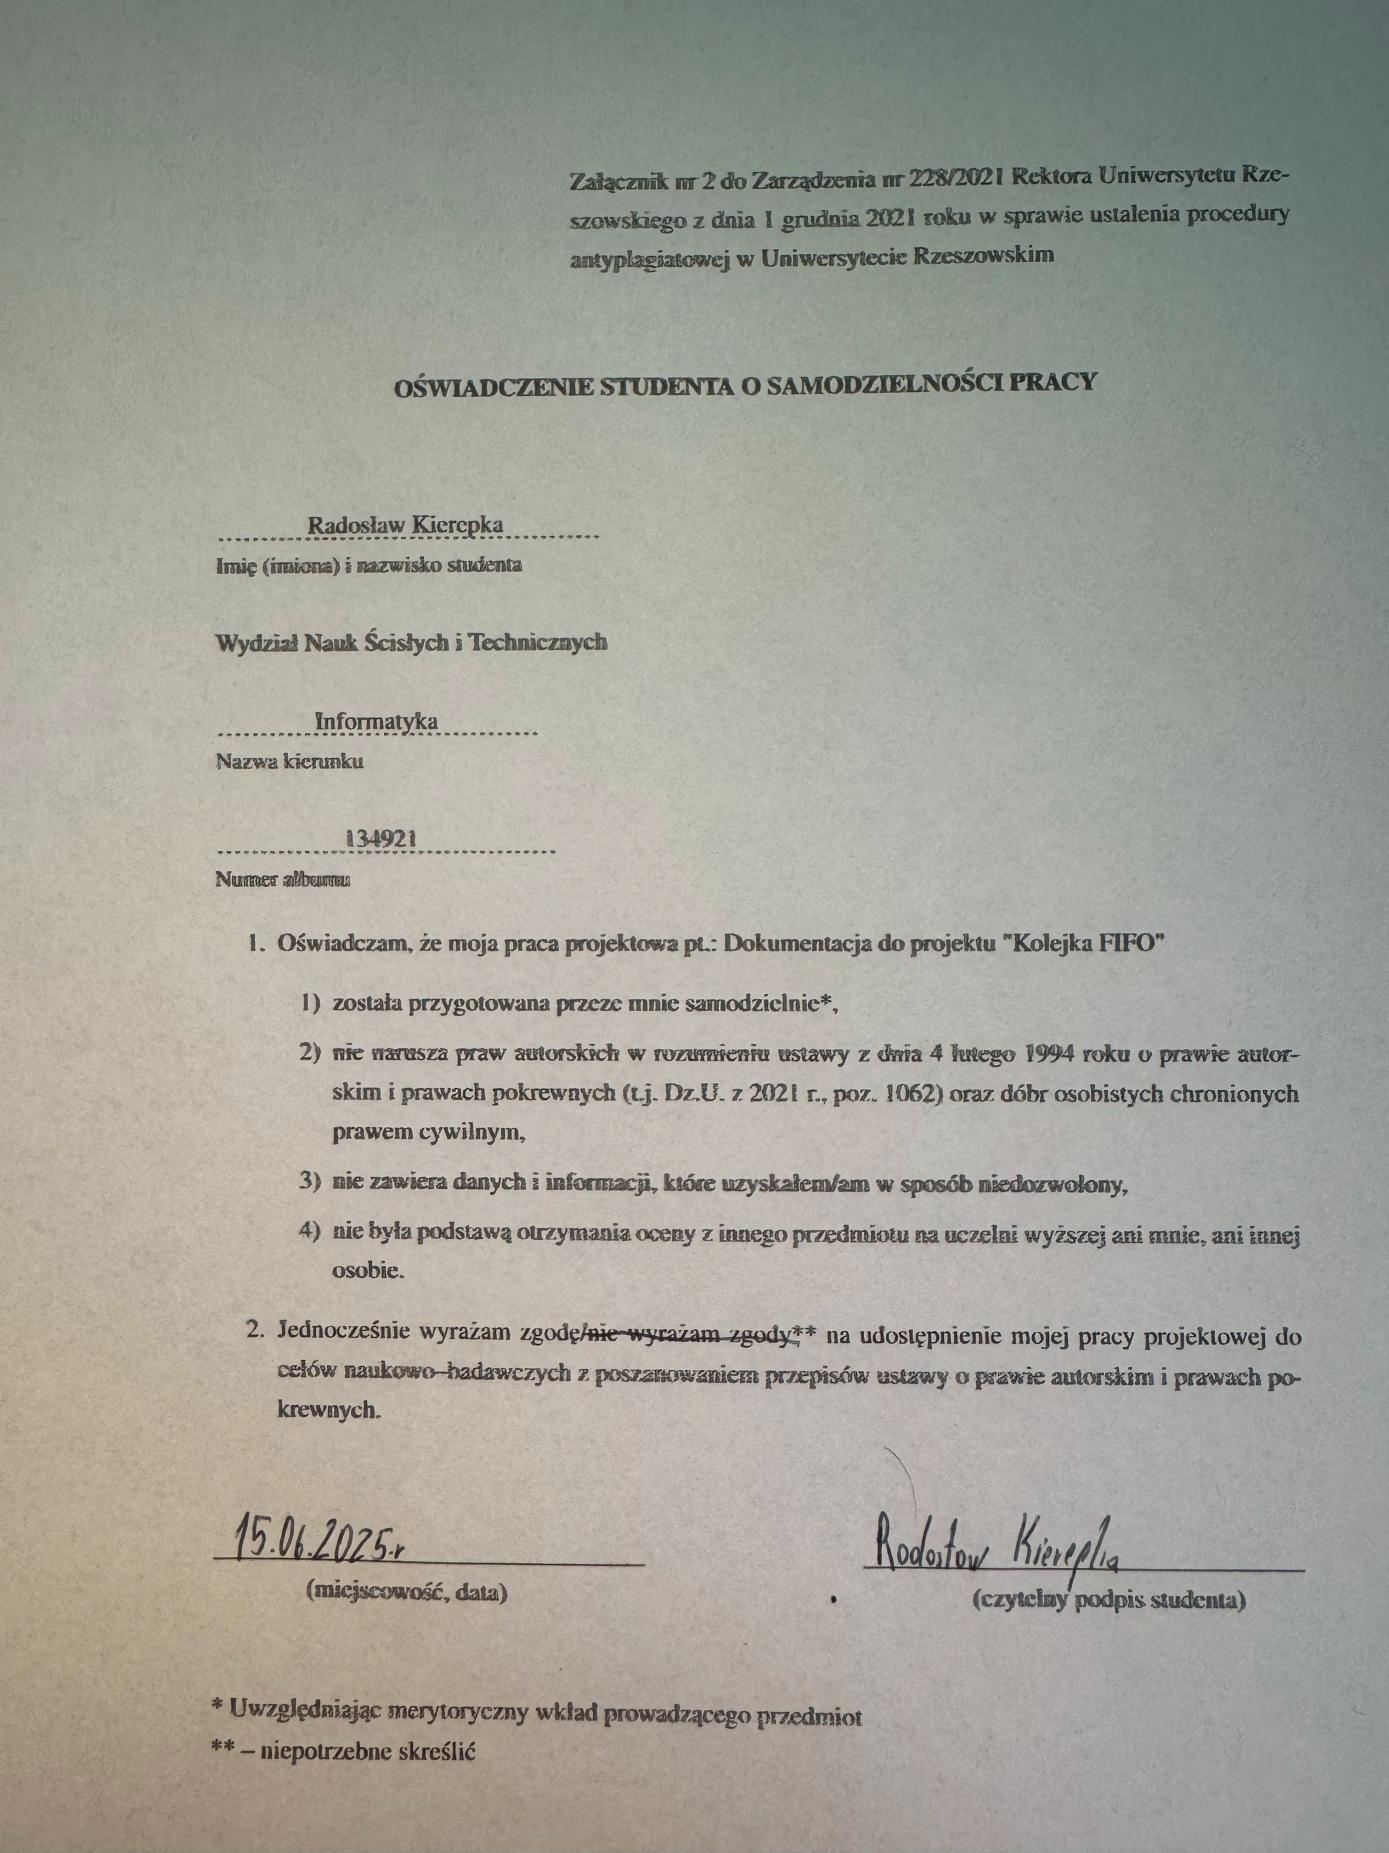
\includegraphics[width=0.7\linewidth]{screenshot001}
	\caption{Oświadczenie studenta o samodzielności pracy}
	\label{fig:screenshot00}
\end{figure}


% ********** Koniec **********